%\documentclass{sensys-proc}
%\documentclass{sig-alternate-ipsn13}
\documentclass{acm_proc_article-sp}
%\documentclass{sig-alternate}
\usepackage{subcaption}
\usepackage{epstopdf}
%\usepackage{times}
\usepackage{hyperref}
\usepackage{multirow}
\usepackage{comment}
%\usepackage[ruled,linesnumbered]{algorithm2e}
\usepackage[ruled]{algorithm2e}
%\usepackage{algorithmic}
%\usepackage{algpseudocode}
\usepackage[yyyymmdd, hhmmss]{datetime}
%\pagestyle{fancy}

\DeclareMathOperator*{\argmax}{arg\,max}
\DeclareMathOperator*{\argmin}{arg\,min}
\newcommand{\mt}{\mathsf{T}}

\begin{document}
\conferenceinfo{BuildSys'13,} {November 14--15, 2013, Rome, Italy} 
\CopyrightYear{2013} 
\crdata{978-1-4503-2431-1/13/11} 
\clubpenalty=10000 
\widowpenalty = 10000

\title{Sensor Type Classification\\ with Transfer Learning Across Buildings
}
\numberofauthors{1} 
\author{
\alignauthor
Dezhi Hong$^1$,  Hongning Wang$^1$,  Kamin Whitehouse$^1$, Jorge Ortiz$^2$\\
	\affaddr{$^1$Department of Computer Science, University of Virginia, VA USA}\\
	\affaddr{$^2$IBM T.J. Watson Research Center, Yorktown Heights, NY USA}\\
	\email{\{hong, hongning, whitehouse\}@virginia.edu, jjortiz@us.ibm.com}
}

\maketitle
\begin{abstract}

TBW

\end{abstract}

\category{C.3}{Special-Purpose And Application-Based Systems}{Real-time and embedded systems}
\terms{Performance, Experimentation, Verification}
\keywords{Building, Sensor Type, Transfer Learning}

% \newpage
\section{Introduction}

To incentivize the reduction of building energy consumption, the U.S. government 
launched the Better Buildings Challenge to make buildings at least 20 percent 
more efficient by 2020~\cite{doe2013better}. To achive this goal, many organizations 
are applying data analytics to the thousands of sensing and control points in 
a typical commercial building to detect wasteful and incorrect operations. These 
complicated analytical processes have proven to be useful and effective on 
a single building, however, an important issue remains that how to make such a process 
generalizable to multiple buildings in a scalable manner. [FIX] need some transition 
before ``however" talking about why we want to port these processes from buildings 
to buildings. On the one hand, analytics-based processes are \emph{tightly coupled} 
to sensors of certain types or locations for each building; on the other hand, 
sensor metadata about the type, location, and relationships between the sensing 
and control units is usually inconsistent across buildings. Therefore, implanting 
these analytical processes requires the correspondence between different naming 
conventions be identified and points be mapped to the inputs of these processes 
before any further analysis is viable. For instance, if A company wants to execute their 
control loops on a building contracted by B company, A needs to first manually 
figure out the mapping of the same type of points between B's system and 
their own system. This process alone can literally take weeks and is proportional 
to the number of points required in the service. Running the same software across 
buildings requires significant integration effort.


\begin{table}[h]
\centering
\begin{tabular}{c|ll}
\cline{1-2}
Building & Point Name & \\
\cline{1-2}
\multirow{2}{*}{\texttt{A}}  & \texttt{Zone Temp 2 RMI204} &  \\
					& \texttt{spaceTemperature 1st Floor Area1} &  \\ \cline{1-2}
\multirow{2}{*}{\texttt{B}} & \texttt{SDH\_SF1\_R282\_RMT} &  \\
                     & \texttt{SDH\_S1-01\_ROOM\_TEMP} &  \\ \cline{1-2}
\multirow{2}{*}{\texttt{C}}  & \texttt{SODA1R300\_\_ART} &  \\
					  & \texttt{SODA1R410B\_ART} &  \\ \cline{1-2}
\end{tabular}
\caption{Example point names for temperature sensors from three different buildings.}
\label{table:ex}
\end{table}


In modern commercial buildings, a sensing or control ``point'' is a sensor
measurement, a controller, or a software value, e.g., a temperature sensor
installed in an office room. The metadata about the point indicates the physical
location, the type of sensor or controller, how the sensor or controller relates
to the mechanical systems, and other important contextual information. Most of
the time, the metadata is encoded as a ``point name'', which is usually a short
text string with several concatenated abbreviations. Table~\ref{table:ex} lists 
a few point names of sensors in three different building management systems contracted 
by Trane\footnote{\url{http://www.trane.com/}}, Siemens\footnote{\url{http://www.siemens.com/}} 
and Barrington Controls\footnote{The company is no longer in business.}. 
For example, the point name \texttt{SODA1R300\_\_ART} is constructed as a
concatenation of the building name (\texttt{SOD}), the air handler unit
identifier (\texttt{A1}), the room number (\texttt{R300}) and the sensor type
(\texttt{ART}, area room temperature). As the name conveys, this point measures 
the temperature in a particular room; and it also indicates the control unit that 
can affect the temperature in this room. Unfortunately, different naming conventions 
are used in most buildings due to different equipment, vendors, manufacturers, 
and contractors being used. As shown in the table, the notion of {\em room temperature} is encoded with a different abbreviation in each of the three buildings: \texttt{Temp}, \texttt{RMT} and \texttt{ART}.
Such variations across different buildings impose great difficulty on scaling up the same analytical process.


Manual normalization of the metadata in buildings becomes intractable due to 
the practical number of buildings. What we often have is one or a few fully 
labeled/normalized buildings. Because the sensor types existing in different buildings 
overlap considerably (e.g., all buildings have temperature sensros installed), it 
would be desirable to leverage the knowledge of one already labeled building to 
help the normalization of a new buidling. 
To abridge the gap between naming conventions for differnt buildings, we envison 
a system that will infer metadata about sensing and control points to a normalized 
common standard.
%based on the knowledge extracted from existing normalized buildings. 
It would allow an advanced analytic engine to quickly connect to and analyze the data 
from a commercial building. Such a system would not only dramatically save time 
but also allow building managers to more easily experiment with many different kinds 
of analytic engines. 
Nevertheless, there is limited work on this topic. 
Bhattarcharya et al~\cite{arka} exploit a programming language based solution, 
where they derive a set of regular expressions from a handful of labeled examples 
to normalize the point name of sensors. 
%This approach assumes a consistent format for all point names, which is not the case in practice, as shown in Table~\ref{table:ex}. 
Schumann et al~\cite{ibm} develop a probabilistic framework to classify sensor types 
based on the similarity of a raw point name to the entries in a manually constructed dictionary. 
%However, the performance of this method is limited by the coverage and diversity of entries listed in the dictionary, and the dictionary size becomes intractable when there exist a lot of variations of the same type, or conflicting definitions of a dictionary entry in different buildings.
Hong et al~\cite{cikm} formulate an active learning based approach to iteratively 
acquire human labels for the building and propogate pseudo labels among points.
However, none of these prior work addresses the scalability issue of metadata 
normalization nor leverages the knowledge from already labeled buildings.

In this work, we demonstrate a first step towards automatic normalization of building 
sensor metadata that requires minimal human intervention. We focus on a key category 
of metadata: the type of a sensing point. In contrast to the aforementioned work, 
where the normalization process is restricted only within the same building, 
we borrow the idea of transfer learning and propose a customized version for transferring 
``knowledge" from an existing building to help infer the sensor type for a new building, which 
effectively minimizes the manual labeling effort throughout the normalization process. 
Based on our observation, the transferral of ``knowledge" is feasible because 
to some extent the actual data of streams carries characteristics that are common 
across buidlings while the point name doesn't. For instance, room temperature 
readings in all buildings are in the range of 60-70 Fahrenheit degree while 
the point names of temperature points can vary a lot according to 
Table~\ref{table:ex}.

To investigate the effectiveness of the proposed solution for sensor type 
classification across buildings, we performed extensive experiments on a large 
collection of real sensor stream data, which includes over 20 different sensor types 
and 3,000 sensors in three different commercial buildings. To our knowledge, we are 
making the first attempt to tackle this problem systematically and our main 
contributions in this paper are as follows:

\begin{itemize}\itemsep1pt \parskip1pt \parsep0pt
\item We empirically analyze how data and point name of the streams can be transferred for classification across buildings.
\item We propose a novel, effective yet general transfer learning approach by exploiting the domain knowledge learnt from an existing building to help the prediction for another building.
\item We evaluate our proposed solution on sensor type classification based on real data and metadata from over 20 different sensor types and 3,000 sensors in three different commercial buildings; and our solution can automatically label at least xx\% of the streams with more than yy\% accuracy without human intervention.
\end{itemize}

%\section{Feature Representation and Transferability}
Two common aspects of the sensor points in a building are the actual data readings and the text string-based point names. Both play an important role for differentiating sensor types.
In this section, we elaborate the construction of two different sets of feature vectors (i.e., data features and name features) and empirically discuss how each of them transfers across buildings in classifying sensor \emph{type}.

\begin{figure*}[ht!]
\centering
  \begin{subfigure}{0.32\textwidth}
                \centering
    \includegraphics[width=\textwidth]{./fig/co2.eps}
                \caption{$CO_{2}$}
  \end{subfigure}
  \begin{subfigure}{0.32\textwidth}
                \centering
    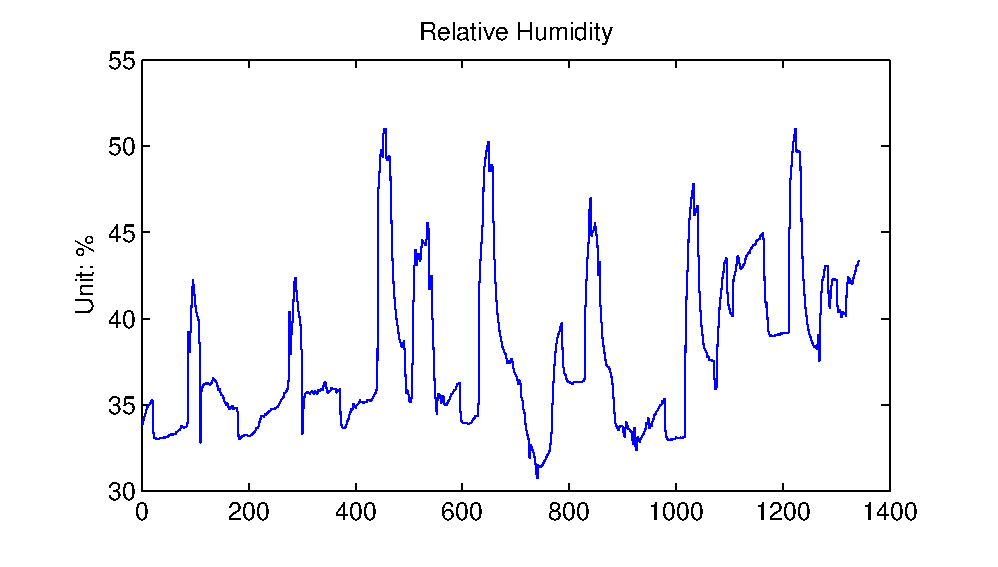
\includegraphics[width=\textwidth]{./fig/rh.eps}
                \caption{Humidity}
  \end{subfigure}
  \begin{subfigure}{0.32\textwidth}
                \centering
    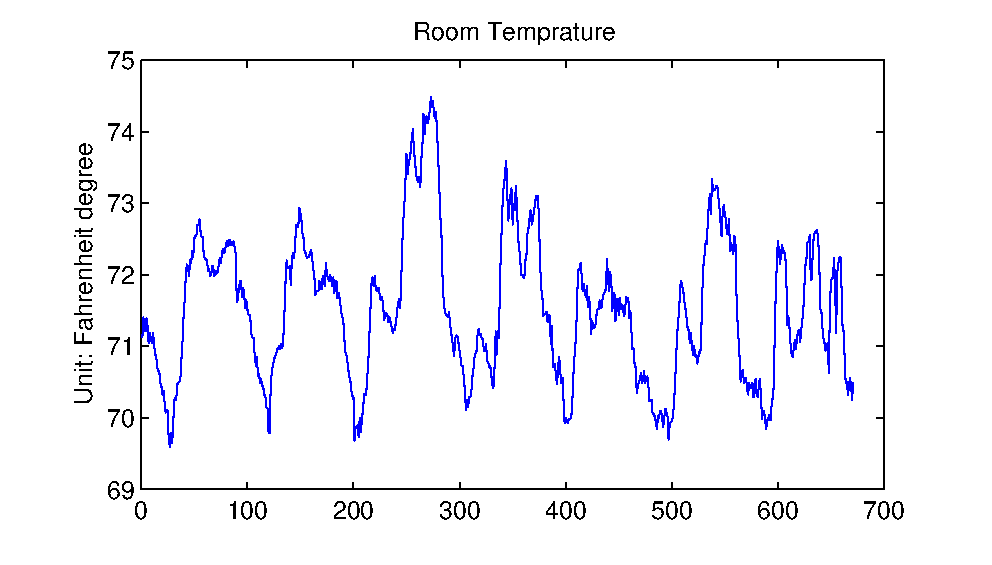
\includegraphics[width=\textwidth]{./fig/rmt.eps}
                \caption{Room Temperature}
  \end{subfigure}
  %row2
  \begin{subfigure}{0.32\textwidth}
                \centering
    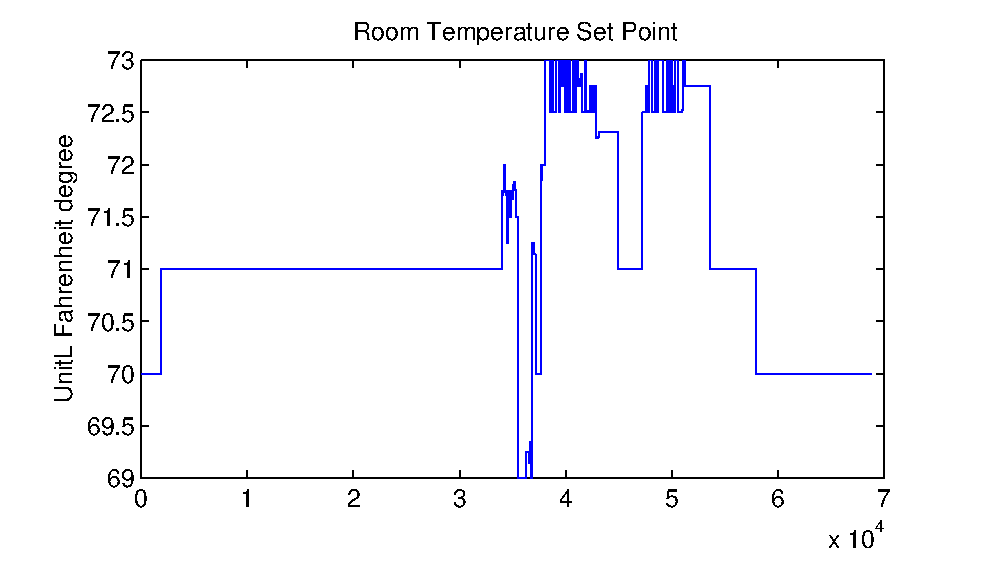
\includegraphics[width=\textwidth]{./fig/stpt.eps}
                \caption{Room Temperature Set Point}
  \end{subfigure}
  \begin{subfigure}{0.32\textwidth}
                \centering
    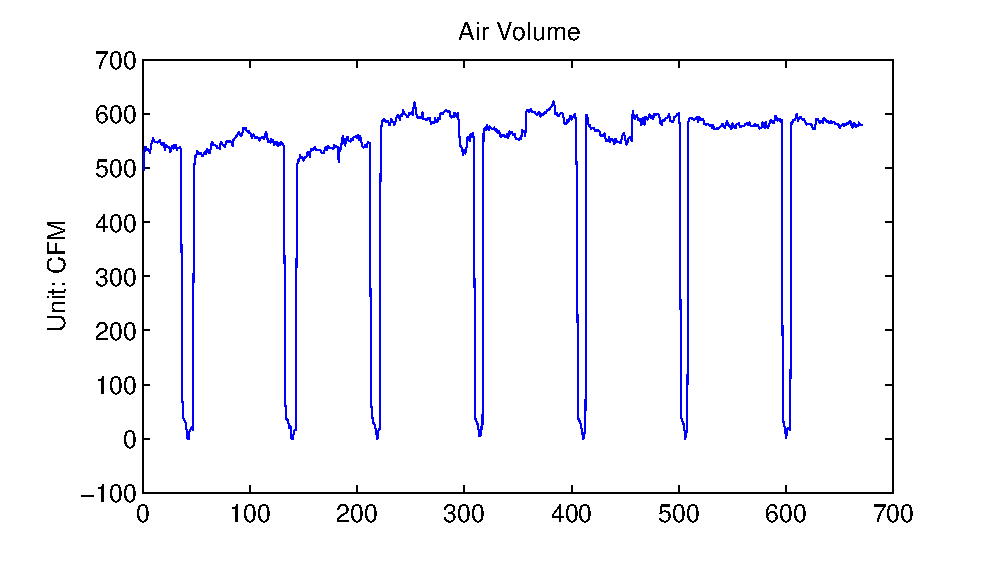
\includegraphics[width=\textwidth]{./fig/vav.eps}
                \caption{VAV Air Volume}
  \end{subfigure}
  \begin{subfigure}{0.32\textwidth}
                \centering
    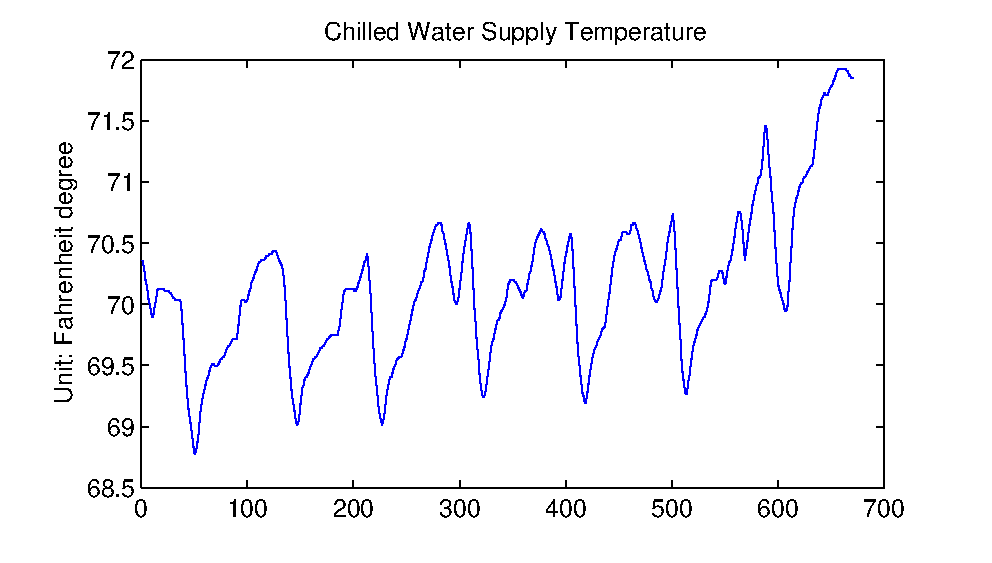
\includegraphics[width=\textwidth]{./fig/cwt.eps}
                \caption{Chilled Water Supply Temperature}
  \end{subfigure}
\caption{Different types of sensors occupy different amplitude bins in the time domain with different short term dynamics.}
\label{fig:example}
\end{figure*}

\subsection{Data Features}
Raw sensor time series\footnote{In this paper, we use the term ``trace'' and ``time series'' \textit{interchangeably}.} usually contain millions of readings which are too many to be useful for type classification. We need to distil the information embedded in the reading patterns.
A signal in the time domain trends the sensor reading and different types of sensor generally occupy distinct amplitude bins, as demonstrated in Figure~\ref{fig:example}. 
We characterize the distribution of a signal in the time domain with standard statistical features, such as the 50th percentile value (also known as the median) as discriminators. 
Table~\ref{table:fd} summarizes the statistical features we used to represent each stream. 


\begin{table}[h]
\centering
\begin{tabular}{r|l|l}
\hline
Category                   & Statistical Function & \multicolumn{1}{l}{Acronym} \\ \hline\hline
\multirow{2}{*}{Extreme}   & Minimum                 & min                          \\ \cline{3-3} 
                           & Maximum                 & max                          \\ \hline
\multirow{2}{*}{Average}   & Median                  & emd                          \\ \cline{3-3} 
                           & Root Mean Square        & rms                          \\ \hline
\multirow{2}{*}{Quartiles} & 1st and 3rd Quartiles   & 1q, 3q                       \\ \cline{3-3} 
                           & Inter-quartile range    & iqr                          \\ \hline
\multirow{3}{*}{Moments}   & Variance                & var                          \\ \cline{3-3} 
                           & Skewness                & skew                         \\ \cline{3-3} 
                           & Kurtosis                & kurt                         \\ \hline
Shape                      & Linear Regression Slope & slope                        \\ \hline
\end{tabular}
\caption{Statistical features extracted in window level for each time series data.}
\label{table:fd}
\end{table}


We segment each sensor readings into an hour-long windows and extract the above features within each window. 
However, computing features over these short time windows will produce too much information as well as noise; too many feature variables typically degrades classifier performance.
To succinctly summarize the dynamics of sensor traces, we compute the statistics of the accumulated features from windowed slices as the final feature set. 
We construct our feature vector as follows: first, each sensor trace is segmented into N non-overlapping one-hour long windows. Second, within each time window, we compute the statistics as in the above table for the trace, producing a vector of each statistical feature after the window slides over the entire trace, such as 
$MIN = \{min^{1}, min^{2}, ..., min^{N}\}$, where N is the number of time windows. Each vector (such as this $MIN$) reflects short term changes but not all the intermediate values are useful for classification. 
Finally, we compute a statistical summary of these vectors. For each vector we compute the minimum, maximum, median and variance, resulting in a feature vector containing 44 variables:
\begin{displaymath}
\begin{split}
F = \{min(MIN), max(MIN), median(MIN), var(MIN),\\
...\\
min(SLOPE), max(SLOPE), median(SLOPE), var(SLOPE)\}
\end{split}
\end{displaymath}
$F$ is the data feature vector for each sensor trace used in our study.


\subsection{Name Features}
The sensor point names are short text strings with several concatenated abbreviations, as shown in our motivating example in Table~\ref{table:ex}. 
To represent the primitive point names as feature vectors for classifier training, we first convert all point names to lower cases and trim out the numerical characters in each point name, resulting in a series of words, e.g., \texttt{Zone Temp 2 RMI204} becomes \texttt{\{zone, temp, rmi\}}. 
To capture possible variants of abbreviations in point names, e.g., ``tmp'' and ``temp'' for temperature, we adopt $k$-mers \cite{leslie2004mismatch} as our features. 
The term $k$-mer refers to all the possible substrings of length $k$, which are contained in a string. This feature is popularly used in protein and gene sequence analysis in bioinformatics, and it helps measure sequence similarity without requiring alignment. 

In our case, we limit the k-mers computation only within a word boundary.
In general, having a too small $k$ will increase the chance for all the k-mers to overlap, making all the points less differentiable.
Therefore, we compute all k-mers of length 3 and 4 for each point name.
For example, \texttt{\{zone, temp, rmi\}} will yield a set of k-mers \texttt{\{zon, one, tem, emp, rmi\}} with $k$=3.
A dictionary of k-mers is constructed with all the k-mers generated from each point name. 
Each point name is converted into a feature vector based on the frequency of k-mers in it. 
For example, a set of k-mers \texttt{\{zon, tem, emp, zon\}} will be transformed to a vector
\texttt{(2,0,1,1,0)} with the dictionary \texttt{\{zon, one, tem, emp, rmi\}}, meaning \texttt{zon} occurs twice, \texttt{one} doesn't appear, and so forth. 
This feature representation of point names will be used for examining classification performance.

\subsection{Transferability}
Now with the two different types of features explained, we examine how well both can perform in classifying sensor types when applied across buildings, i.e., learning a classifier based on the features from building A and testing it on building B. 
Intuitively, data features should be more generalizable than point names with respect to differentiating points by types. 
This is because in general a certain type of sensors will share commonality in reading amplitude and trend, such as diurnal patterns. 
For example, temperature readings in a building will be between 60-70 degree with rises in the morning and falls at night.
In contrast, point name features might not transfer well due to various naming conventions across buildings as shown in Table~\ref{table:ex}.
Although k-mers can enlarge the size of term dictionary in a building to increase the chance of covering more terms in other buildings, such a technique still cannot fundamentally compensate for the difference in naming conventions.

\begin{table}[h]
\centering
\begin{tabular}{l|c|c}
\hline
                & Data Feature & Name Feature \\ \hline
A-\textgreater B & 0.778       & 0.341       \\
B-\textgreater A & 0.612       & 0.328       \\ \hline
\end{tabular}
\caption{Type classification accuracy between two buildings with different sets of features.}
\label{table:clf}
\end{table}


To empirically examine how well each type of feature transfers, we perform type classification across buildings with both features in separate. With either set of features from building A, we train a linear SVM and apply it to building B on the same type of feature, or vice versa. Table~\ref{table:clf} summarizes the results.
We see that data features do transfer better than name features as expected, but the results from data features still contain significant errors making them far from being usable. 
The question remains how to better leverage these two sources of information from one building and transfer them to another.
We will discuss the idea of transfer learning in next section.



\section{Transfer Learning}
In this work, we employ a transfer learning to classify sensor types for a building with the knowledge from another labeled building. Both data features and name features are used to accomplish the classification task: an ensemble of base learners are constructed with data features and applied to the other building because data features transfer across buildings, while the clustering structure on name features in the other building is exploited to help determine which base classifier should contribute more in predictions. 
To accommodate the variations in point names, we appeal to a non-parametric Bayesian approach to identify the clustering structure.


\subsection{Knowledge Transfer}
The use of transfer learning is motivated by the fact that people often have one or only a few buildings labeled of which they want to take advantage to aid the labeling of a new buidling.
In our sensor type classification setting, we assume that we are provided with some labeled examples only from the training domain but do not have any labeled ones from the testing domain. 
Transfer learning fits such a scenario well in that it exploits knowledge gained from one domain\footnote{A ``domain'' particularly refers to a data set  in this paper.} where labeled data is abundant to help classify examples in a new related domain. 
Such knowledge transfer is possible when the training domain and the test domain have the same set of class labels. 
The reason that traditional supervised learning techniques is not successful in transferring knowledge across domains in our case is because it usually requires training and the testing examples sampled i.i.d. from the same distribution, which is not the case for our problem.

%For example, the classiers can be trained from several relevant domains or built using different learning algorithms on the same domain.
Based on the observation in Section x.x that classifiers constructed with data features perform better than name features when applied across buildings, we construct a few classifiers with different learning algorithms on the same set of data features from an existing building. 
Each different classifier usually contains a different perspective of the knowledge on the building, due to the inductive bias of the specific learning model. 
We refer to these different classifiers as {\it base} models\footnote{We use the term ``model'' and ``classifier'' {\it interchangeably} in this paper.} and will combine them for classification on the new building.

\subsection{Locally Weighted Ensemble}
Different models can be effective at different regions or structures in the new testing building, and no single model can perform well on all examples. 
Ideally, we want to combine the knowledge in the base models, rather than only using any particular model, to more effectively transfer the knowledge to the new building. A natural choice is model averaging that additively combines the predictions of multiple base learners. 
However, the existing model averaging methods for traditional supervised learning usually assign global weights to models, which are either uniform (e.g., in Bagging~\cite{bagging}) or proportional to the training accuracy (e.g., in Boosting~\cite{boosting}), or simply relying on a specific model (e.g., single model classification).
Such global weighting schemes may not perform well in transfer learning because different testing examples may favor predictions from different base models. 
For example, when the base models carry conflicting concepts at a testing example, the optimal choice would be a model that better represents the distribution underlying the example.

We employ a locally weighted ensemble~\cite{lwe} to weight the predictions from base classifiers. 
The weight is computed per model per example based on the similarity between the model and the local structure of the target example. The similarity is measured by comparing neighborhood graphs which we will explain in the next section. Such local weighting will favor models whose predicted local structure is close to the true local structure of the target example in the new testing domain. Let $x$ be the data feature vector of an example in the new building and $y$ be its predicted class label. Given a set of $k$ base models $M_1, \dots, M_k$ and the new testing set $D_T$ represented in the data feature view, the general Bayesian model averaging rule to estimate the posterior distribution of $y$ is,
\begin{equation}\label{eq_lwe}
p(y|x)=\sum_{i=1}^k p(y|x,D_T,M_i) p(M_i|D_T)
\end{equation}
where $p(y|x,D_T,M_i) = p(y|x,M_i)$ because $x \in D_T$ and $p(y|x,M_i)$ is actually the prediction on $x$ by $M_i$. And $p(M_i|D_T)$ is the probability to choose $M_i$ given the testing set $D_T$. As $x \in D_T$, $p(M_i|D_T)$ equals to $p(M_i|x)$ which is the locally adjusted weight for $M_i$ and Eq.~\ref{eq_lwe} becomes,
\begin{equation}\label{eq_sum}
p(y|x)=\sum_{i=1}^k w_{x}^{M_i} p(y|x, M_i)
\end{equation}
where $w_{x}^{M_i} = p(M_i|x)$ and intuitively, a model $M_i$ should have higher weights for $x$ if $M_i$ predicts a similar local structure of $x$ to the true one.
We will next explain how the weight is calculated per example.

\subsection{Graph-based Weight Estimation}\label{sec:gwe}
If $p(y|x)$ is known, we can estimate the weights $w_{x}^{M_i}$ for each model by minimizing the square error between its prediction and the ground truth. 
However, in practice the truth value of $p(y|x)$ for a new building is not available a priori . 
The main task becomes to properly define the similarity between classifier's predicted structure and the true structure. 
Based on the clustering assumption~\cite{cluster} that $p(y|x)$ is not expected
to change much in a dense area where $p(x)$ is high, which means the decision boundary probably exists in areas with smaller $p(x)$.
Therefore, we perform clustering on the new testing set and assume the boundaries between clusters represent areas where $p(x)$ is small.
If the clustering boundary for the region where $x$ locates agrees with the decision boundary of $M_i$, we assume that $p(y|x,M_i)$ is similar to the true $p(y|x)$ around $x$, which means we can assign a larger weight to $M_i$ at $x$. 
In other words, if the predictions of $M_i$ on the area surrounding $x$ have higher consistency with the clustering results, $M_i$ would have a larger weight at $x$. 

Following these observations, we employ a graph-based algorithm to compute the weight.
To compute the $w_{x}^{M_i}$ for $M_i$ at example $x$, we construct two neighorhood graphs: 
$G_M = (V, E_M)$ and $G_C = (V, E_C)$, for classification and clustering respectively, 
where each vertex is an example and $V = D_T$. In $G_M$, an edge exists between two vertices (denoting the two examples are ``neighbors'') if and only if $M_i$ predicts the same label for these two examples. Likewise, in $G_C$, an edge exists between two vertices if and only if these two examples reside in the same cluster.
If the neighbors of $x$ on both graphs significant overlap, then $M_i$ will be assigned a larger weight.
So the weight $w_{x}^{M_i}$ for $M_i$ at $x$ is proportional to the similarity of the two graphs:
\begin{equation}\label{eq_sim}
w_{x}^{M_i} \propto s(G_M, G_C|x) = \frac {|V_M \cap V_C|} {|V_M \cup V_C|}
\end{equation}
where $V_M$ ($V_C$) is the set of neighbors of $x$ on graph $G_M$ ($G_C$), |$\cdot$| is the cardinality of a set, and $s(G_M, G_C|x)$ is the similarity between two graphs. 
Figure~\ref{fig:graph} illustrates an example of neighborhood graphs for an example $x$ (in grey circle): model 1 has a similarity of 0.75 while model 2 has 0.5.

\begin{figure}[h]
\centering
    \includegraphics[width=0.4\textwidth]{./fig/lwe_graph}
\caption{An example of local neighborhood graphs of $x$ (in grey circle).}
\label{fig:graph}
\end{figure}

With Eq.~\ref{eq_sim} defined, we can compute the weight for each $M_i$ by normalizing among all similarity scores:
\begin{equation}\label{eq_norm}
w_{x}^{M_i} = \frac {s(G_{M_i}, G_C|x)} {\sum_{i=1}^k s(G_{M_i}, G_C|x)}
\end{equation}
And the final prediction for $x$ is simply $\hat y = argmax_y \enspace p(y|x)$ as $p(y|x)$ is defined in Eq.~\ref{eq_sum}.

\subsubsection{Distance-based Adjustment}
We notice in some cases the original similarity definition can be problematic. Consider the case as shown in Figure~\ref{graph_dist}, there are two neighbors on both of the graphs for the two models and the distance between vertices are marked on the edge. Since the original similarity definition only considers the number of neighbors, both models will be assigned the same weight of 0.5 in this case while obviously model 1 ought to have a higher weight because the neighbors on
the left graph are closer to the target example.
To fix the issue, we include the distance between examples into consideration, the adjusted similarity is:
\begin{equation}\label{d_sim}
s^\ast(G_M, G_C|x) = 1 - \frac {\sum d_{V_I}/|V_I|} {\sum d_{V_U}/|V_U|}
\end{equation}
where $V_I = V_M \cap V_C$, $V_U = V_M \cup V_C$, and $\sum d_{V_I}$ is the sum of distance between $x$ to its neighbors in $V_I$ (likewise for $\sum d_{V_U}$).

\begin{figure}[h]
\centering
    \includegraphics[width=0.4\textwidth]{./fig/lwe_d_graph}
\caption{An example of local neighborhood graphs of $x$ with distance into consideration.}
\label{graph_dist}
\end{figure}

\subsubsection{Thresholding-based Adjustment}
The use of weighted average decision for $x$ among base classifiers is reasonable when at least some of these classifiers perform well on $x$. However, the similarity $s(G_{M_i}, G_C|x)$ for $M_i$ is expected to be small when the predictions of $M_i$ around $x$ conflict with its true local structure. 
In such a case, still adopting the decision from the classifier might not be a reasonable choice. 
Since $s(G_{M_i}, G_C|x)$ reflects the consistency between classifier predictions and cluster structure, we use the average similarity score over all $M_i$ on $x$ as a discriminator to limit the usage of these base classifiers.
As an adjustment before the normalization of similarity scores, we check the average similarity score with,
\begin{equation}\label{ave_sim}
 \bar s_x = \frac {1}{k}\sum_{i=1}^k s(G_{M_i}, G_C|x)
\end{equation}
We will continue with the ensemble prediction only if $\bar s_x$ is larger than a threshold $\delta$, and we will discuss the choice of $\delta$ in the evaluation section.


\subsection{Clustering with Non-parametric Bayesian}
\label{sec_clustering}
In our transfer learning based approach, data density $p(x)$ is exploited via its latent clustering structure. We choose Gaussian Mixture Model (GMM) \cite{zivkovic2004improved}, a partitional clustering algorithm, to perform the clustering.

In GMM, the cluster label for every instance is treated as a latent variable, which is drawn from a multinomial distribution $p(c)$, i.e., $p(c)\propto\alpha_c$, where $\forall c, \alpha_c\ge0$ and $\sum_c\alpha_c=1$. In any given cluster $c$, the conditional data likelihood of an instance $x$ is specified by a multivariate Gaussian distribution. To reduce the number of parameters to estimate, we choose the isotropic Gaussian in our solution,
\begin{equation}
p(x|c)=(2\pi\sigma^2)^{-d/2}\exp{-\frac{(x-\mu_c)^\mt (x-\mu_c)}{2\sigma^2}}
\end{equation}
where the variance $\sigma^2$ is shared by all the clusters. $\{\alpha_c, \mu_c\}^k_{c=1}$ and $\sigma$ are considered as model parameters in GMM.

However, in GMM, we need to manually specify the number of clusters for a given input data set; and the clustering result of GMM is very sensitive to such setting. More importantly, in our study, usually there is more than one pattern in the point names even for the same type of sensors; therefore we cannot assume one class has only one cluster. It is impossible for us to predefine those optimal cluster sizes. To make clustering feasible on the new building, we appeal to a non-parameter Bayesian solution: we assume the model parameters $(\alpha, \mu)$ in each cluster are also random variables, which are drawn from a Dirichlet Process prior \cite{dp}.

A Dirichlet Process $DP(G_0, \eta)$ with a base distribution $G_0$ and a scaling parameter $\eta$ is a distribution over distributions~\cite{dp}. The base distribution $G_0$ specifies the prior distribution of model parameters, e.g., mean parameter $\mu$ in each cluster, and the scaling parameter $\eta$ specifies the concentration of samples drawn from the DP, e.g., cluster proportion $p(c)$. An important property of the DP is that though the draws from a DP have countably infinite size, they are discrete with probability one, which leads to a probability distribution on partitions of the data. The number of unique draws, i.e., the number of clusters, varies with respect to the data and therefore is random, instead of being pre-specified.

As a result, with the introduced $DP(G_{0}, \eta)$ prior, data density in a given collection of instances can be expressed using a stick-breaking representation
\cite{sethuraman1994constructive}:
\begin{equation}\label{eq_dp_density}
p(x)=\sum_{c=1}^\infty \alpha_c \mathcal{N}(x|\mu_c,\sigma)p(\mu_c|G_0)
\end{equation}
where $\alpha={\alpha}_{c=1}^\infty\sim Stick(\eta)$ represents the proportion of clusters in the whole collection. The stick-breaking process $Stick(\eta)$ for the cluster proportion parameter $\alpha$ is defined as: $\alpha'_c\sim Beta(1, \eta), \alpha_c=\alpha'_c\prod_{i=1}^{c-1}(1-\alpha'_i)$. Since the variance $\sigma^2$ is fixed in all clusters, we use a conjugate prior for $\mu$ in $G_0$, i.e., for $\forall c, \mu_{ci}\sim \mathcal{N}(a,b)$, with the assumption that each dimension in $\mu_c$ is independently drawn from a univariate Gaussian. This will greatly simplify the later on inference procedure.

Because the data density distribution defined in Eq~\eqref{eq_dp_density} only has finite support at the points of $\{\alpha_c, \mu_c\}^k_{c=1}$, we can calculate the posterior distribution of latent cluster labels in each unlabeled instance to discover the clustering structure. Following the sampling scheme proposed in \cite{neal2000markov}, we appeal to a Gibbs sampling method to infer the posterior of cluster membership. Detailed specifications of this sampling algorithm can be found in \cite{neal2000markov}.

\subsubsection{Features for Clustering}
We use point name features to generate clusters for the new building. In general, point names following the same pattern would not vary too much, which will yield clusters of higher quality than data features.
Table~\ref{quality} shows the quality of clusters generated by DP with data features and name features measured by rand index~\cite{rand}. Rand index is a standard measure of the similarity between the grouping in clusters and the true labels.

\begin{table}[h]
\centering
\begin{tabular}{l|c|c}
\hline
                & Data Feature & Name Feature \\ \hline
Rand Index & 0.34       & 0.75       \\ \hline
\end{tabular}
\caption{Quality of clusters generated with different features measure by rand index (in the range [0,1], higher is better).}
\label{quality}
\end{table}

{\bf Putting it all together:} Algorithm~\ref{algo} summarizes our transfer learning algorithm for the sensor type classification across buildings. We start from training a few base classifiers with the data features and labels of examples in a source building. We also generate clusters with DP on the name features of examples in the target building. For each example $x$ in the target building, we measure the local similarity score for each base classifier. If the average similarity is significant enough, we compute the weight for each classifier at $x$ by normalizing the similarity score. Finally we calculate the weighted sum of predictions from all base classifier and obtain the label $y$ for $x$.

\begin{algorithm}[ht]
 \caption{Transfer Learning for Sensor Type Classification}
 \label{algo}
 %\SetAlgoLined
 {\bf Input}: Data features of the source building $\mathcal{D_S}=\{x^D_1,x^D_2,\dots,x^D_n\}$ and their labels $\mathcal{Y_S}=\{y_1,y_2,\dots,y_n\}$  data features of the target building $\mathcal{D_T}=\{x^D_1,x^D_2,\dots,x^D_m\}$, and name features of the target building $\mathcal{P_T}=\{x^P_1,x^P_2,\dots,x^P_m\}$\\
 {\bf Output}: predicted labels of the examples in target building $\mathcal{Y}$\\
 Initialize: Generate clusters with $DP(G_{0}, \eta)$ on $\mathcal{P_T}$\\
 Train $k$ classifiers $M_1, \dots, M_k$ based on $\mathcal{D_S}$ and $\mathcal{Y_S}$\;

\For{$x^D$ in $\mathcal{D_T}$}{
Construct neighborhood graphs $G_M$ and $G_C$ for $x^D$ as defined in Section~\ref{sec:gwe} for each $M_i$;\\
Compute the similarity score for each $M_i$ with Eq.~\ref{d_sim};\\
Check the average similarity score $\hat s_x$ over all $M_i$ with Eq.~\ref{ave_sim};\\
If $\hat s_x > \delta$, then use Eq.~\ref{eq_norm} and Eq.~\ref{eq_sum} to predict the label $y$;
}
\end{algorithm}


\section{Evaluation}
To demonstrate the effectiveness of our method, we evaluate our transfer learning based classification technique on actual data and point names of sensors from three commercial buildings. Extensive experiments demonstrate that our technique is able to accurately classify by type for a considerable portion of examples without human intervention. We also discuss how the threshold parameter $\delta$ on similarity score affect the learning accuracy and also explain the decision of how to set such a parameter.

\subsection{Taxonomy and Data Collection}
\begin{figure}[t]
\centering
\includegraphics[width=0.38\textwidth]{./fig/hvac}
\caption{A typical HVAC system consisting of an air handler unit (AHU), several variable air volume boxes (VAV), water-based heating/cooling pipes and air circulation ducts. (Figure used with permission from the authors of~\cite{sentinel}.)}
\label{fig:hvac}
\end{figure}

Figure~\ref{fig:hvac} illustrates a typical heating, ventilation, and air conditioning (HVAC) system deployed in modern commercial buildings. 
An HVAC system usually uses a combination of hot and cold water pipes in conjunction with
air handler units (AHU) to maintain the appropriate thermal environment within the building.
An HAVC system usually consists of several AHUs and each AHU is responsible for a physical zone
in the building. An AHU consists of variable speed drives that supply cold air
(cooled by the supplied cold water) using ducts to VAV boxes distributed throughout the building.
The hot water loop is also connected to these VAV boxes using separate pipes. Each VAV box
controls the amount of air to be let into an HVAC zone using dampers, whose opening angle
can be programmed. A reheat coil, which uses supplied hot water, is used to heat the air to
meet the appropriate HVAC settings for each zone.

Table~\ref{table:num} summarizes all the types of sensors evaluated in our analysis in these three buildings and the number of sensors of each type. ``Room temperature'' measures the temperature in room and for a better understanding, all the other temperature measurements on water circulation and air ventilation are illustrated in Figure~\ref{fig:hvac}. For setpoints, we assign only
one general type which includes all set points for every actuator configured in the building.

Our evaluation data set containing both data and point names of sensor streams is collected from over 2,500 sensors of different types deployed in three commercial buildings. 
We collected a week's worth of data from each building.
Specially, Building A is the Rice Hall at the University of Virginia, where the sense points report to a database by Trane anywhere between every 10 seconds to every 10 minutes.
Both building B and C are from UC Berkeley: B is the Sutardja Dai Hall with sensors and equippment from KETI~\cite{keti} and Siemens~\cite{bacnet}, while building C is the Soda Hall what uses an archaic system by Barrington Controls which is no longer in business. 
Points and sensors in these two buildings transmit data to an archiver~\cite{smap} periodically from anywhere between every 5 seconds to every 10 minutes.


\begin{table}[t]
\centering
\begin{tabular}{l | l l l}
\hline
& \multicolumn{3}{c}{Building} \\
Type & A & B & C\\
\hline\hline
$CO_{2}$ & 16 & 52 & 0\\
Humidity & 54 & 52 & 0\\
Air Pressure & 142 & 216 & 215\\
Room Temp & 159 & 231 & 208\\
Facility Operation Status & 59 & 72 & 41\\
Facility Control & 0 & 138 & 403\\
Setpoint & 140 & 486 & 229\\
Air Flow Volume & 14 & 172 & 9\\
Damper Position & 0 & 290 & 10\\
Fan Speed & 0 & 25 & 15\\
HW Supply Temp & 27 & 1 & 0\\
HW Return Temp & 15 & 1 & 0\\
CW Supply Temp & 18 & 2 & 11\\
CW Return Temp & 15 & 3 & 10\\
Supply Air Temp & 20 & 17 & 3\\
Return Air Temp & 6 & 2 & 4\\
Mixed Air Temp & 5 & 2 & 3\\
Ice Tank Entering Temp & 1 & 2 & 0\\
Ice Tank Leaving Temp & 1 & 4 & 0\\
Occupancy & 25 & 52 & 0\\
Timer & 0 & 0 & 15\\ \hline
Sum & 575 & 1124 & 1166\\ \hline
\end{tabular}
\caption{Number of points by type for the 3 test buildings. ``Temp" stands for ``temperature", ``HW" for ``hot water" and ``CW" for ``cold water".}
\label{table:num}
\end{table}


All of our learning and classification processes are implemented based on the scikit-learn~\cite{scikit} library, which is an open-source machine learning package 
implemented mostly in Python providing a rich set of APIs.

\subsection{Base Classifiers and Baseline}
\label{sec:baseline}
Our transfer learning based approach exploits a few base classifiers. Each base classifier will be trained on the same set of data features from the source building in a general way, therefore there is no particular requirement on what classifiers should be selected here.
Particularly, we employ three base classifiers: Ranfom forest, linear regression and support vector machines with RBF kernels.


\begin{figure*}[ht!]
\centering
  \begin{subfigure}{0.32\textwidth}
                \centering
    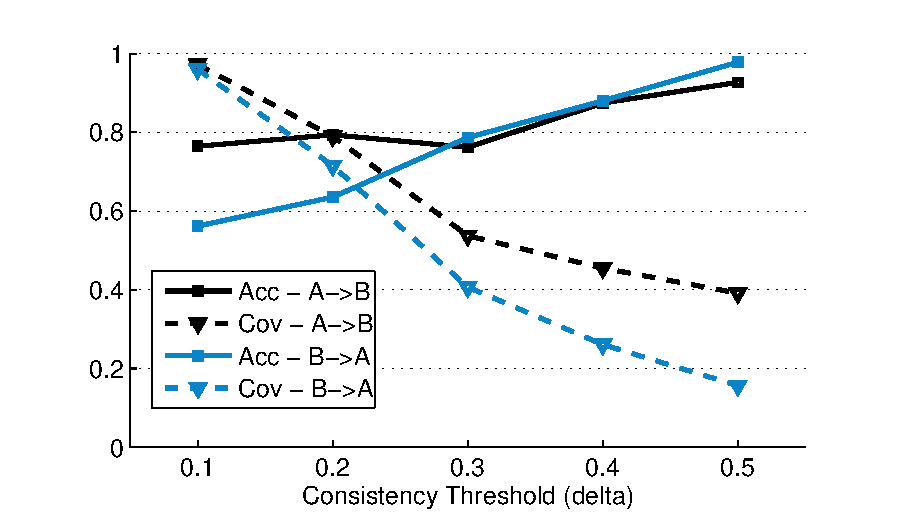
\includegraphics[width=\textwidth]{./fig/TL_AB.eps}
                \caption{A and B}
  \end{subfigure}
  \begin{subfigure}{0.32\textwidth}
                \centering
    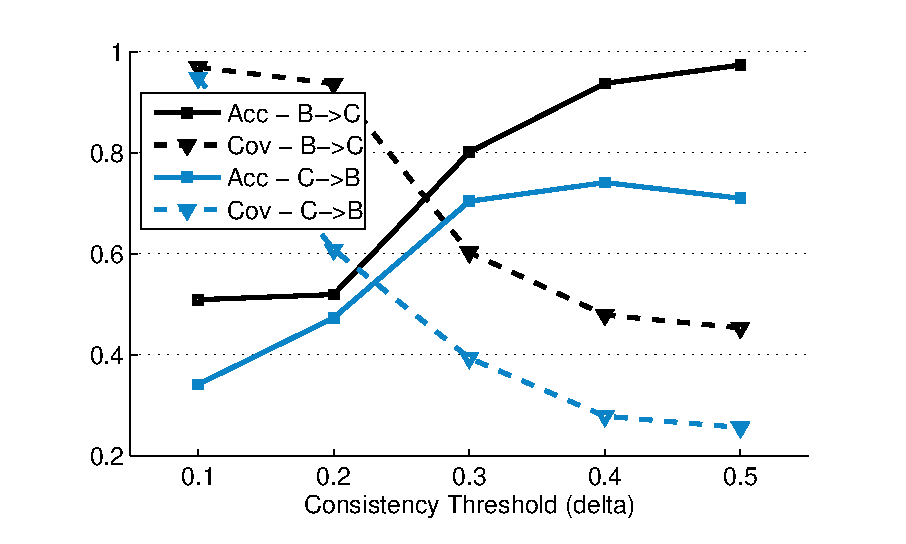
\includegraphics[width=\textwidth]{./fig/TL_BC.eps}
                \caption{B and C}
  \end{subfigure}
  \begin{subfigure}{0.32\textwidth}
                \centering
    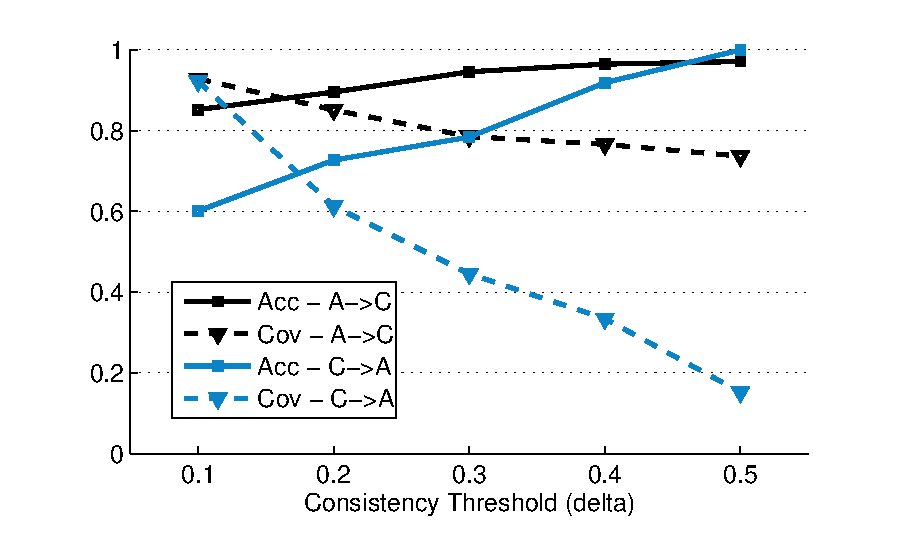
\includegraphics[width=\textwidth]{./fig/TL_AC.eps}
                \caption{A and C}
  \end{subfigure}
\caption{Type classification accuracy against labeled percentage with transfer learning between different pairs of buildings.}
\label{fig:tl_acc}
\end{figure*}


As a baseline to compare our proposed approach against, we adopt a 


For classification, we measure the averaged cross-validation accuracy in two different scenarios (intra- and inter- buildings). In the intra-building case, the 
data from a single building is split into training and testing sets, where the results illustrate how accurately the type information can be inferred using local 
within-building information. For inter-building case, the experiment performs training and testing across buildings, i.e, train the classifier on the data from building A 
and test it on building B.  
This set of experiments tests how well we can apply the classification boundaries from one building and apply it to another.

\subsection{Base Classifier Performance}
In the table, each row is specific to a \emph{type} and each column is the \emph{percentage} of the full data set that was used for training.
Each cell shows two values.  
\begin{table}[h]
\centering
\begin{tabular}{r|c|c|c}
\hline
 & A     & B     & C     \\ \hline
A & N/A   & 1/2/3 & 1/2/3 \\ \hline
B & 1/2/3 & N/A   & 1/2/3 \\ \hline
C & 1/2/3 & 1/2/3 & N/A   \\ \hline
\end{tabular}
\caption{Base classifier performance across buildings on data features. The three numbers are for random forest, logistic regression and SVM respectively.}
\label{acc_base}
\end{table}

\subsection{Transfer Learning Accuracy}
We investigate the overall accuracy of transfer learning for type classification across our three testing buildings. There are three pair of choices and for each pair the transferral can be done either way, therefore, we have six testing case. The classification results is illustrated in Figure~\ref{fig:tl_acc}.

\subsection{Exploitation of Labels in the New Building}


%\section{Discussion}
There are several aspects of our work that we left out or did not have time to explore more deeply.
First we go over the expansion of \emph{type} classes and how we could increase coverage of sensor types in future work. 
We discuss how we could improve classification accuracy
by looking for data sources outside the building data sets. We also discuss why principal component analysis is an aspect that we
did not explore in depth and how the principal components can change from building to building.  Finally, we 
explain how our misclassification identifier could be used to improve classification results.

\textbf{Unlabeled Streams}

\textbf{Complementing Traditional Labeling}

\textbf{Better Features for Classifiers}
The performance of transfer learning and classification processes in our work is bounded by the base classifiers which rely only on a set of general features. The line of work to represent time series with discretized symbols (e.g., the SAX~\cite{sax}) or primitive ``shapes'' (e.g., the ``shapelets''~\cite{shapelet1, shapelet2}) doesn't work well for our problem due to the variability in ``shapes'' and unpredictable human noises. There, we wish to explore how using external or domain-specific knowledge could help improve the classification accuracy. 

\textbf{Multiple Buildings as Source}




\section{Related Work}
There has been much research work on sensor stream clustering and trace analysis.

Much work adopts random forest on xxx.

\section{Conclusion}
We describe a general, simple yet effective feature extraction design in support of sensor type classification with time series data. By experimenting 
with over 2000 streams from two buildings on two campuses, our technique, which leverages an ensemble learning method, is able to achieve an accuracy more than 
92\% and 82\% for testing within building and across buildings, respectively. We also discuss that how to choose the window size applied 
to a slice of the original time series and how the number of training instances affects classification accuracy. In general, around 100 instances are 
enough to bootstrap the learning process in the case of 6 types of sensors. Another important contribution of our paper is a probability-based solution for identifying 
potentially misclassified instances. With the use of probabilities produced by the random forest, in both of the intra- and inter- building learning cases, we are able 
to identify at least 30\% of the misclassifications.% with an overhead of inspecting some actual correct classification as well.

Our technique can act as a tool for metadata construction for building sensors. For cases where type information of sensors is missing, our technique can 
help infer and generate the type metadata. In cases where metadata is available in an inconsistent manner within/across buildings, our solution 
can be used to verify type information and unify the naming schema across platforms in different buildings. Questions remain about how broadly we 
can expand our taxonomy and further study the scalability of our technique.

% is before it becomes a generally viable solution to building metadata construction.

%\section{Acknowledgements}
%Thanks to our shepherd, Kin Cheong Sou, and the anonymous reviewers for helpful comments. Thanks to Albert Goto, for making the first author's stay at UC Berkeley comfortable. Sincere gratitude goes to Kamin and David, for letting this collaboration happen. This work was partly funded by the NSF grants EFRI-1038271 and CPS-1239552.
\bibliographystyle{abbrv}
\small
%\footnotesize
\bibliography{buildsys}

%\balancecolumns
\end{document}
